\documentclass[12pt,a4paper]{article}

\usepackage[utf8]{inputenc}
\usepackage[ngerman]{babel}
\usepackage[T1]{fontenc}
\usepackage{amsmath}
\usepackage{amsfonts}
\usepackage{amssymb}
\usepackage{graphicx}
\usepackage[left=2cm,right=2cm,top=2cm,bottom=2cm]{geometry}
\usepackage{multicol}
\usepackage{booktabs}
\usepackage[hidelinks]{hyperref}
\usepackage{tikz}
\usepackage{pgfplots}
\usepackage{blindtext}
\usepackage{array}
\usepackage{multirow}
\usepackage{bigdelim}
\usepackage{colortbl}
\usepackage{fancyhdr} 
\usepackage{tabularx}
\usepackage{xcolor}
\usepackage{color}
\usetikzlibrary{decorations.text}
\usetikzlibrary{tikzmark}
\pagestyle{fancy} 
	\fancyhf{} 
	\fancyhead[L]{
\includegraphics[scale=0.05]{Bilder/dhbw.png}} 
	\fancyhead[C]{\slshape Projektmanagement} 
	\fancyhead[R]{\slshape LaTeX Version}

\usepackage{helvet}
\renewcommand{\familydefault}{\sfdefault}

\author{\slshape Robin Rausch, Florian Maslowski}
\title{Projektmanagement}
\date{\slshape \today}
\begin{document}
\maketitle
\tableofcontents
\newpage
\section{Fragenkatalog}
\begin{enumerate}
\item Wie ist ein Projekt definiert (Eigenschaften)?
	\begin{enumerate}
	\item[] Einmaligkeit der Bedingungen 
	\item[] Zielvorgabe 
	\item[] Begrenzungen von Ressourcen (Zeit, Finanzen, Personal)
	\item[] Abgrenzung zu anderen Vorhaben 
	\item[] Projektspezifische Organisation 
	\end{enumerate}
\item Was ist Projektmanagement?
	\begin{enumerate}
	\item[] Führungskonzept zur zielorientierten Durchführung großer Vorhaben 
	\item[] Gesamtheit der Führungsaufgaben 
		\begin{enumerate}
		\item[*] Zielsetzung
		\item[*] Planung
		\item[*] Steuerung
		\item[*] Überwachung
		\end{enumerate}
	\item[] Führungsaufbaus (Projektorganisation)
	\item[] Führungstechnik (Führungsstil) 
	\item[] Führungsmittel (Methoden) 
	\end{enumerate}
\item Warum gehen Projekte schief?
	\begin{enumerate}
	\item[] Unklare Definition der Projektziele und Aufgaben 
	\item[] Falsche Einschätzung von Risiken 
	\item[] Verschiedene Projekt Vorstellungen die nicht abgestimmt werden  
	\item[] Ungenügende Kommunikation im Team 
	\end{enumerate}
\item Was ist die Aufgabe eines Projektmanagers?
	\begin{enumerate}
	\item[] Aufgabenverteilung und Priorisierung 
	\item[] Kommunikation zwischen Gruppen 
	\item[] Ziele festlegen und erreichen  
	\item[] Konfliktbewältigung 
	\item[] Sicherstellung der Wirtschaftlichkeit  
	\item[] Entscheidung über Inhalt und Projektablauf 
	\end{enumerate}
\item Welches sind die drei Säulen der PRM-Kompetenz?
	\begin{enumerate}
	\item[] Fachliche Kompetenz 
	\item[] Wirtschaftliche Kompetenz 
	\item[] Soziale Kompetenz
	\end{enumerate}
\item Wozu dient das PM-BoK?
	\begin{enumerate}
	\item[] Kann Firmenspezifisch angewendet werden 
	\item[] Informationen über die Wissensgebiete im Projektmanagement  
		\begin{enumerate}
		\item[*] Integrationsmanagement
		\item[*] Umfangsmanagement
		\item[*] Terminmanagement
		\item[*] Kostenmanagement
		\item[*] Qualitätsmanagement
		\item[*] Personalmanagement
		\item[*] Kommunikationsmanagement
		\item[*] Risikomanagement
		\item[*] Beschaffungsmanagement
		\end{enumerate}
	\end{enumerate}
\item Wozu benötigt man Ziele im Projekt und wie unterteilt man diese?
	\begin{enumerate}
	\item[] Um den Soll-Zustand festzustellen (Was soll erreicht werden?) 
	\item[] Unterteilung in: 
		\begin{enumerate}
		\item[*] Funktionale Ziele (Qualitative Ziele)
		\item[*] Operationale Ziele (Quantitative Ziele)
		\end{enumerate}
	\end{enumerate}
\item An welches Prinzip sollten sich Ziele anlehnen?
	\begin{enumerate}
	\item[] SMART: 
		\begin{enumerate}
		\item[*] S: Spezifisch
		\item[*] M: Messbar
		\item[*] A: Angemessen
		\item[*] R: Realistisch
		\item[*] T: Terminierbar
		\end{enumerate}
	\end{enumerate}
\item Welche Ziele dienen zur Messung des Erfolgs eines Projekts?
	\begin{enumerate}
	\item[] Sachziele
	\item[] Terminziele
	\item[] Kostenziele
	\end{enumerate}
\item Was versteht man unter dem magischen Dreieck im PRM?
	\begin{enumerate}
	\item[] Zirkuläre Abhängigkeiten
	\item[] \includegraphics[scale=0.3]{Bilder/magischesDreieck.PNG}
	\end{enumerate}
\item Was ist ein Zielsystem?
	\begin{enumerate}
	\item[] Ein Oberziel wird in mehrere Ziele unterteilt
	\end{enumerate}
\item Verschiedene Projektorganisationen
	\begin{enumerate}
	\item[] Einfluß Projektmanagement
		\begin{enumerate}
		\item[]
		\end{enumerate}
	\item[] Matrix Projektmanagement
		\begin{enumerate}
		\item[]
		\end{enumerate}
	\item[] Reines Projektmanagement
		\begin{enumerate}
		\item[] 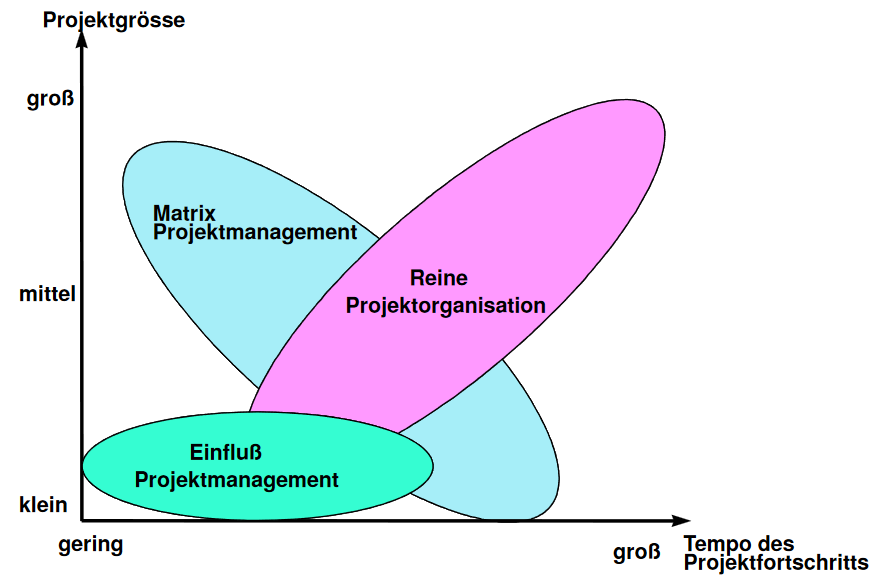
\includegraphics[scale=0.6]{Bilder/projektorganisationenWirksamkeit.PNG}
		\end{enumerate}
	\end{enumerate}
\end{enumerate}

\end{document}